\documentclass[9pt]{beamer}

% \usepackage[T1]{fontenc}
\usepackage[utf8]{inputenc}
\usepackage[russian]{babel}
\usepackage{graphicx}
\usepackage{hyperref}
\graphicspath{ {images/} }

\usetheme{Goettingen}


\title{Использование сонаров для решения задачи картографирования в мобильной робототехнике}

% A subtitle is optional and this may be deleted
% \subtitle{Optional Subtitle}

% \author{Денис Шепелев\inst{1}}
\author{Денис Шепелев}

% - Give the names in the same order as the appear in the paper.
% - Use the \inst{?} command only if the authors have different
%   affiliation.

\institute[Universities of Somewhere and Elsewhere] % (optional, but mostly needed)
{
  % \inst{1}%
  % 073а\\
  ИППИ РАН \\ МФТИ
}
% - Use the \inst command only if there are several affiliations.
% - Keep it simple, no one is interested in your street address.

\date{58 научная конференция МФТИ, 2015}
% \date{}

\begin{document}

\begin{frame}
  \titlepage
\end{frame}

% \begin{frame}{Outline}
%   \tableofcontents
%   % You might wish to add the option [pausesections]
% \end{frame}

% Section and subsections will appear in the presentation overview
% and table of contents.


% \begin{frame}{Name}
% \begin{columns}
%   \begin{column}{0.50\textwidth}
%     \begin{itemize}
%       \item
%       {
          
%       }
%     \end{itemize}
%   \end{column}
%   \begin{column}{0.50\textwidth}
%     \begin{figure}[h]
%       \centering
%       \includegraphics[width=0.8\textwidth]{name.png}
%     \end{figure}
%   \end{column}
% \end{columns}

% \end{frame}

\section{2D карты и датчики}

\subsection{2D карта}

\begin{frame}{2D карта}
\begin{columns}
  \begin{column}{0.50\textwidth}
    \begin{itemize}
      \item
      {
        Карта - обычное изображение.
      }
      \item
      {
        Каждый пиксель - некоторая область пространства.
      }
      \item
      {
        Белый пиксель - свободная для движения область. 
      }
      \item
      {
        Черный - чем-то занятая облать.
      }
      \item
      {
        Серый - неизвестная область.
      }
    \end{itemize}
  \end{column}
  \begin{column}{0.50\textwidth}
    \begin{figure}[h]
      \centering
      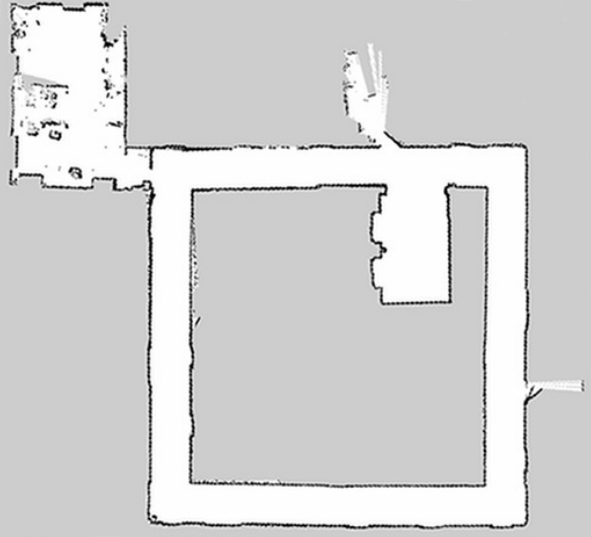
\includegraphics[width=0.8\textwidth]{grid_map.png}
    \end{figure}
  \end{column}
\end{columns}
\end{frame}

\subsection{Датчики}

\begin{frame}{Датчики}

\begin{itemize}
  \item
  {
    Сонары.
  }
  \item
  {
    Лидары.
  }
  \item
  {
    Стереокамеры.
  }
\end{itemize}

\end{frame}


% \begin{frame}{Name}
% \begin{itemize}
%   \item
%   {
      
%   }
% \end{itemize}
% \end{frame}

\subsection{Задача 2D картографирования}

\begin{frame}{Задача 2D картографирования}
\textbf{Дано}:
\begin{itemize}

  \item
  {
    Есть данные датчиков.
  }
  \item
  {
    Известно положение робота, в любой момент времени.
  }
\end{itemize}
\textbf{Цель}:
\begin{itemize}
  \item
  {
    Построить карту с учетом вышесказанного.
  }
\end{itemize}
\end{frame}

\begin{frame}{Датчики}

\begin{itemize}
  \item
  {
    Сонары.
    \begin{itemize}
    \item
    {
      Достаточно точны для широкого круга задач.
    }
    \item
    {
      Отностиельно дешевые.
    }
    \end{itemize}
  }
  \item
  {
    \textcolor{red}{Лидары}.
  }
  \item
  {
    \textcolor{red}{Стереокамеры}.
  }
\end{itemize}

\end{frame}

\section{Подходы к решению задачи}

\subsection{Подходы к решению задачи}

\begin{frame}{Подходы к решению задачи}
Различают два основных подхода к решению задачи 2D картографирования:
\begin{itemize}
  \item
  {
    с обратной моделью сенсора

    $$P(m|z)$$
  }
  \item
  {
    с прямой моделью сенсора

    $$P(z|m)$$
  }
\end{itemize}

\end{frame}

\subsection{Алгоритм с обратной моделью сенсора}

\begin{frame}{Алгоритм с обратной моделью сенсора}

\begin{itemize}
  \item
  {
    Итеративный алгоритм
  }
  \item
  {
    Каждая ячейка обновляется по формуле

    \begin{equation}
      \begin{split}
        \frac{P(m_i | z_{1:t}, x_{1:t})}{1 - P(m_i | z_{1:t}, x_{1:t})} = 
        \frac{P(m_i | z_t, x_t)}{1- P(m_i | z_t, x_t)}\\
        \frac{P(m_i | z_{1..t-1}, x_{1:t-1})}{1- P(m_i | z_{1..t-1}, x_{1:t-1})}\\
        \frac{1 - P(m_i)}{P(m_{i})}
      \end{split}
    \end{equation}
  }
\end{itemize}
\end{frame}

\begin{frame}{Алгоритм с обратной моделью сенсора}

\begin{itemize}
  \item
  {
    Отлично подходит для лидаров
  }
  \item
  {
    Не подходит для работы с сонарами
  }
\end{itemize}
\end{frame}


\begin{frame}{Алгоритм с обратной моделью сенсора}
При получении формулы (1) предполагается, что
$P(z_t|m_{ij}, z_{1:t}) = P(z_t|m_{ij})$ - для сонаров плохая аппроксимация

\begin{columns}
\begin{column}{0.33\textwidth}
  \begin{figure}[h]
    \centering
    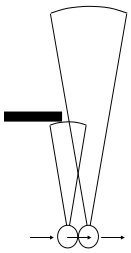
\includegraphics[width=0.65\textwidth]{inv1.png}
  \end{figure}
\end{column}
\begin{column}{0.33\textwidth}
\begin{figure}[h]
    \centering
    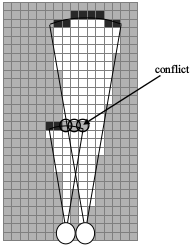
\includegraphics[width=0.9\textwidth]{inv2.png}
\end{figure}
\end{column}
\begin{column}{0.33\textwidth}
  \begin{figure}[h]
    \centering
    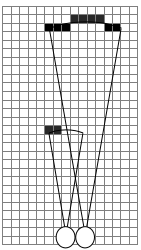
\includegraphics[width=0.7\textwidth]{inv3.png}
  \end{figure}
\end{column}
\end{columns}
\end{frame}

\begin{frame}{Алгоритм с обратной моделью сенсора}
TODO вставть рисуночер с нашими результатами
\end{frame}

\subsection{Алгоритм с прямой моделью сенсора}
\begin{frame}{Алгоритм с прямой моделью сенсора}
\begin{itemize}
  \item
  {
      
  }
\end{itemize}
\end{frame}

% \begin{frame}{Name}
% \begin{itemize}
%   \item
%   {
      
%   }
% \end{itemize}
% \end{frame}


% All of the following is optional and typically not needed. 
\appendix
\section<presentation>*{\appendixname}
\subsection<presentation>*{Источники}

\begin{frame}[allowframebreaks]
  \frametitle<presentation>{Источники}
    
  \begin{thebibliography}{10}
    
  % \beamertemplatebookbibitems
  % Start with overview books.

  % \bibitem{ LL }
  %   Wolfram Burgard, Diego Tipaldi
  %   \newblock {\url{http://ais.informatik.uni-freiburg.de/teaching/ss15/robotics/slides/17-3dmapping.pdf}}

  %   \newblock {\em Материалы лекции Фрайбургского университета по курсу Introduction to
  %   Mobile Robotics - Techniques for 3D Mapping}.
 
  % \beamertemplatearticlebibitems
  % % Followed by interesting articles. Keep the list short. 

  % \bibitem{OctoMap}
  %   Armin Hornung, Kai M. Wurm, Maren Bennewitz, Cyrill Stachniss, Wolfram Burgard
  %   \newblock {OctoMap:
  % An Efficient Probabilistic 3D Mapping Framework Based on Octrees}
  %   \newblock {\em Autonomous Robots April 2013, Volume 34, Issue 3, pp 189-206}

  % \bibitem{MLS}
  %   Rudolph Triebel, Patrick Pfaff, Wolfram Burgard
  %   \newblock {Multi-Level Surface Maps for Outdoor Terrain Mapping and Loop Closing}
  %   \newblock {\em In Proceedings of the IEEE/RSJ International Conference on Intelligent Robots and Systems (IROS ’06)}

  \end{thebibliography}
\end{frame}

\end{document}


